\chapterimage{analisis.jpg} % Table of contents heading image
\chapter{Análisis del sistema e interacción}

La interacción del sistema se puede visualizar mediante diagramas de secuencia, con los cuales se podrá hacer un análisis más clarificado sobre cómo es el ciclo de vida del programa y de qué forma son las relaciones internas de éste.

Para detallar un poco más sobre la comunicación de las partes del sistema, es indispensable un diagrama de comunicación, en donde se podrá detallar los que se transmite entre los objetos, es similar al diagrama de secuencia pero no describe un orden de transmisión de mensajes sino que se centra en los mismos mensajes dados.

Por ultimo, para aclarar cómo se compone el sistema, se explicarán los diagramas de clases, éstos describen cómo están conformadas las calases del sistema, cómo son sus relaciones y sobretodo, cuales son los patrones de diseño que se implementan en la aplicación y cómo optimizan el  funcionamiento de la misma.

%%%%%%%%%%%%%%%%%%%%%% Sección 4.1 %%%%%%%%%%%%%%%%%%%%%%%%%%%
\section{Diagramas de secuencia}

Un diagrama de secuencia muestra una interacción, que representa la secuencia de mensajes entre instancias de clases, componentes, subsistemas o actores. El tiempo fluye por el diagrama y muestra el flujo de control de un participante a otro. Utilice diagramas de secuencia para visualizar instancias y eventos, en lugar de clases y métodos. En el diagrama, puede aparecer más de una instancia del mismo tipo. También puede haber más de una ocurrencia del mismo mensaje \cite{Pw3DS}.

Un diagrama de secuencia es aquel en el que se muestra la interacción entre actores, objetos, interfaces, controles, bases de datos y otras entidades a través del tiempo según el enfoque, el cual puede ser:
\begin{itemize}
	\item \textbf{Enfoque de objetos}: donde son participes las relaciones que existen entre éstos y con actores para realizar una tarea determinada.
	\item \textbf{Enfoque de modelado a tres capas}: donde el actor se comunica con una entidad interfaz, y ésta a su vez con una entidad control para llegar a una persistencia. 
\end{itemize}

Es importante resaltar que cada diagrama de secuencia se realiza en torno a la descripción de un caso de uso dado, ya que éste define el orden en que se deban distribuir las tareas para cada una de las entidades que son participes a la hora de representar cada caso.

Para este proyecto se realizaron 5 casos de uso de los cuales se va a crear un diagrama de secuencia por cada caso y uno para cada enfoque. Inicialmente el caso de uso de .

A continuación se describirá cada diagrama de secuencia:

\paragraph{Diagrama del control de asistencia}

\begin{figure}[H]
	\centering
	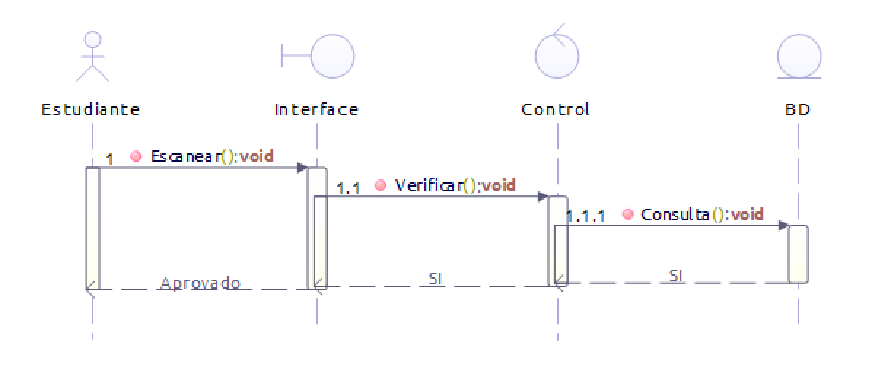
\includegraphics[width=1\linewidth]{parte2/imgs/DiagramaSecuencia/Asistencia}
	\caption[Diagrama de secuencia de registro de Asistencia]{Diagrama de secuencia para el registro del control de asistencia}
	\label{fig:diagramadesecuencia1}
\end{figure}
Este diagrama de secuencia explica el funcionamiento del programa frente al control de asistencia de los estudiantes al apoyo alimentario.
\\
Para este caso el estudiante representa el usuario que ingresa al programa y que mediante el escaneo del codigo del carnet realiza la actualizacion de asistencia en la base de datos.

 





\paragraph{Diagrama del Registro de usuarios}
\begin{figure}[H]
	\centering
	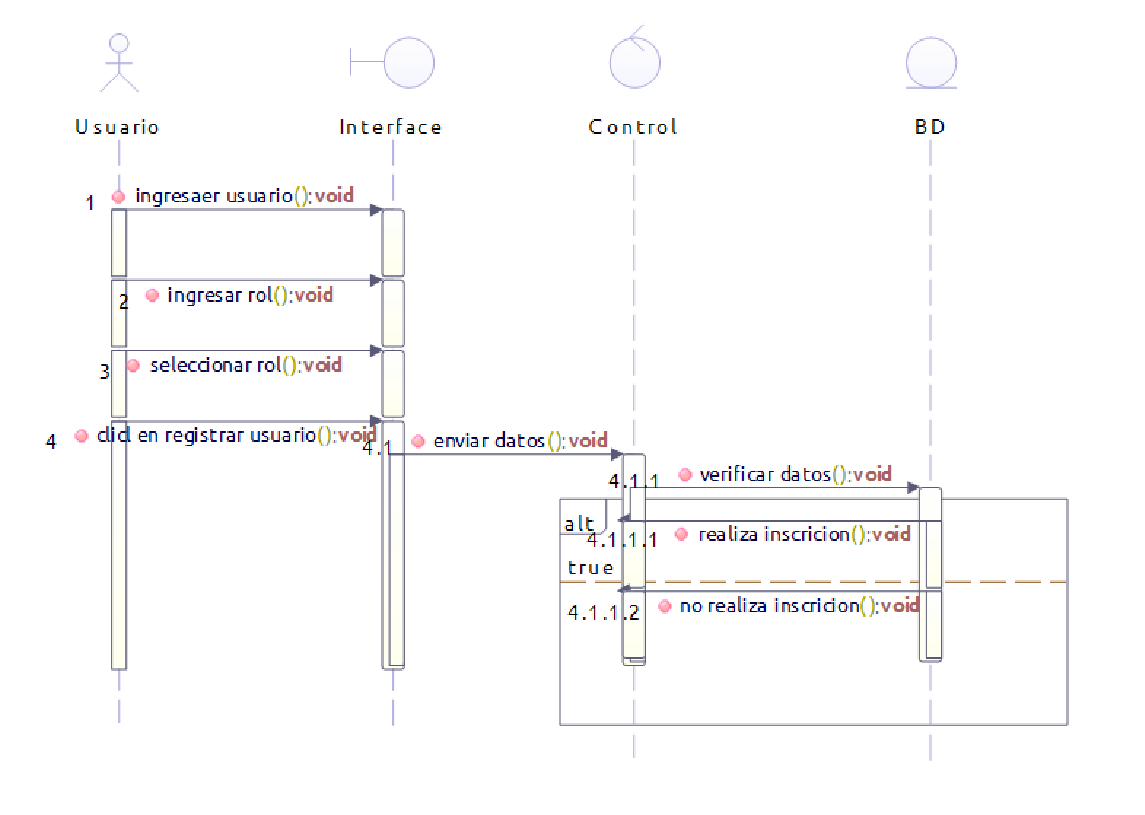
\includegraphics[width=0.8\linewidth]{parte2/imgs/DiagramaSecuencia/RegUsu}
	\caption[Diagrama de secuencia Registrar Usuario]{Diagrama de secuencia para el registro de usuarios}
	\label{fig:diagramadesecuencia2}
\end{figure}

Este diagrama de secuencia representa el registro de un usuario. Para lo cual el usuario ingresa sus datos selecciona un rol y realiza el click para registrar los datos y consulta dentro de la base de datos la existencia del usuario y si existe se envia un mensaje que alerta sobre la existencia del usuario. 



\paragraph{Diagrama para crear nuevas convocatorias}
\begin{figure}[H]
	\centering
	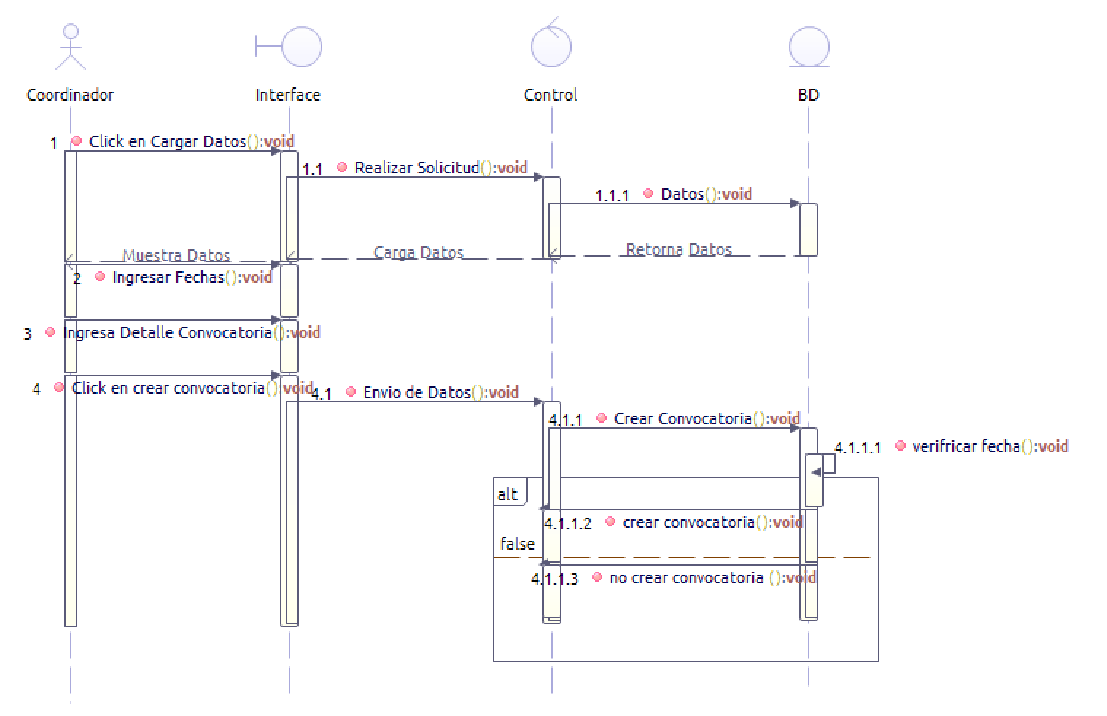
\includegraphics[width=0.8\linewidth]{parte2/imgs/DiagramaSecuencia/SecCrearConv}
	\caption[Diagrama de secuencia Crear convocatoria]{Diagrama de secuencia para crear una nueva convocatoria}
	\label{fig:diagramadesecuencia5}
\end{figure}
Este diagrama de secuencia representa el registro de convocatorias de apoyo alimentario dentro del aplicativo.El programa registra los datos para los cuales nescesita realizar la carga  datos, fechas y detalles especificos de cada convocatoria que al final mediante una consulta a la base de datos define si se puede crear o no la convocatoria.


 
\paragraph{Diagrama del registro a convocatoria existentes}
\begin{figure}[H]
	\centering
	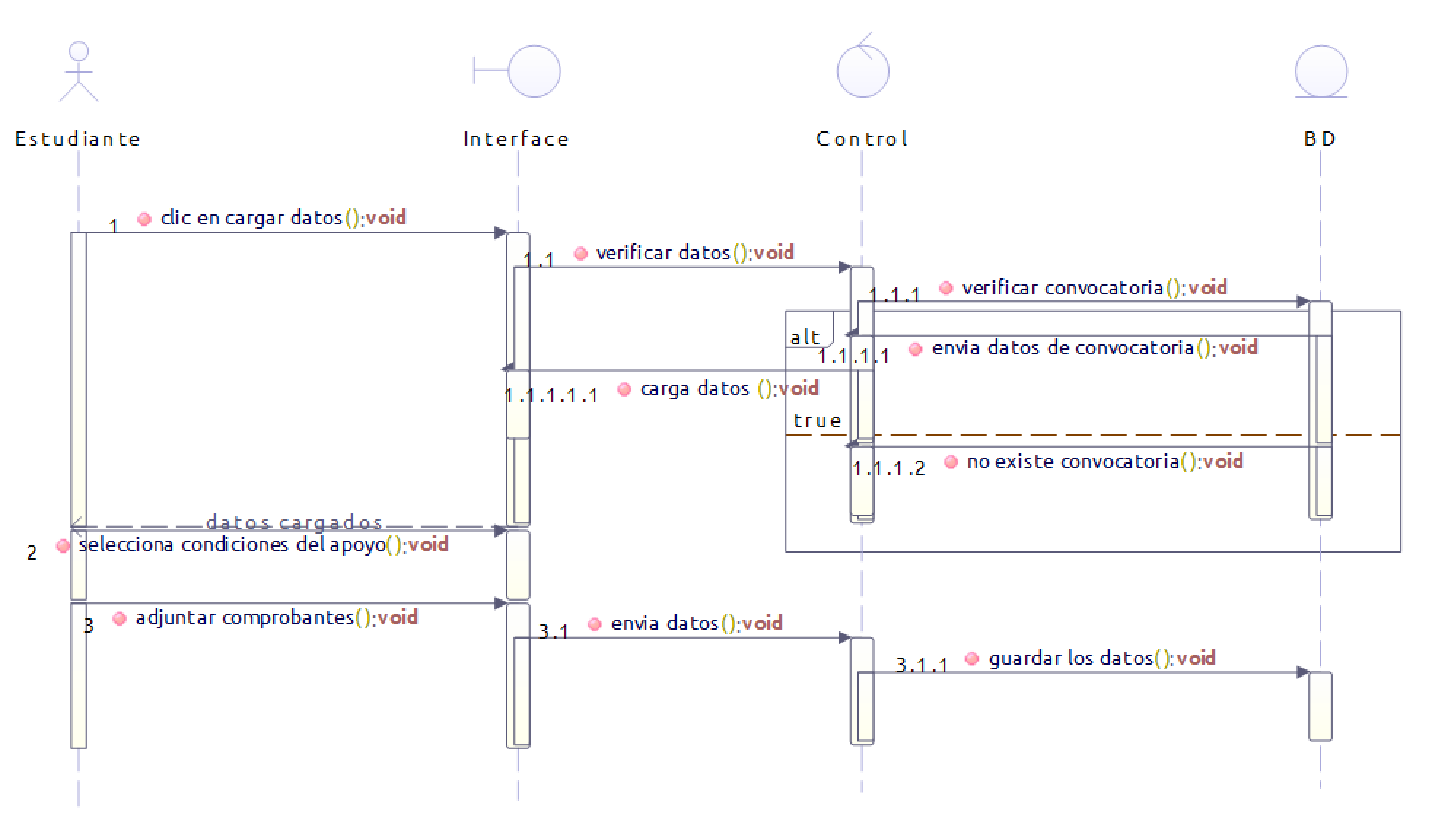
\includegraphics[width=0.8\linewidth]{parte2/imgs/DiagramaSecuencia/SecSolConv}
	\caption[Diagrama de secuencia Registro a una convocatoria]{Diagrama de secuencia para el registro a una convocatoria}
	\label{fig:diagramadesecuencia3}
\end{figure}

En este diagrama se realiza la solicitud de los usuarios a una nueva convocatoria. Para este proceso es nescesario que los usuarios carguen toda la informacion que luego se registra en la base de datos.


\paragraph{Diagrama de la verificacion de una solicitud a una convocatoria}
\begin{figure}[H]
	\centering
	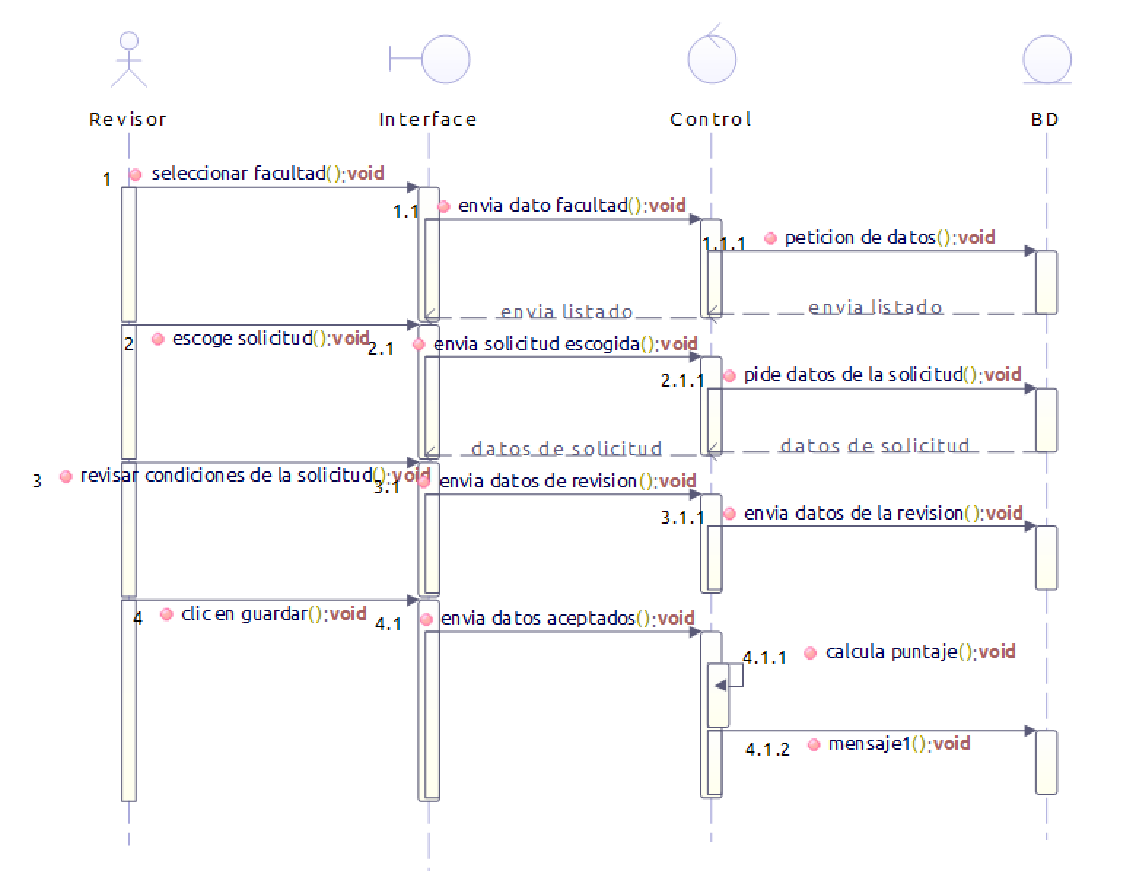
\includegraphics[width=0.8\linewidth]{parte2/imgs/DiagramaSecuencia/SecVerifSolConv}
	\caption[Diagrama de secuencia Verificacion de solicitud]{Diagrama de secuencia de verificacion de una solicitud a una convocatoria}
	\label{fig:diagramadesecuencia4}
\end{figure}

Para este diagrama representamos la intereaccion que tiene un usuario revisor con las solicitudes presentes en la base de datos. En este caso el revisor realiza la seleccion de la facultad y se muestra un listado de las solicitudes de dicha facultad y se escoge la solicitud y consulta en la base de datos la solicitud escogida. Envia los datos de la revision y los datos aceptados a los cuales le calcula el puntaje y envia los datos a la base de datos

\newpage

%%%%%%%%%%%%%%%%%%%%%% Sección 4.2 %%%%%%%%%%%%%%%%%%%%%%%%%%%
\section{Diagramas de comunicación}

También llamados Diagramas de Colaboración. Nos sirven para enfatizar los vínculos de datos entre los participantes de una interacción. Un diagrama de Comunicación modela las interacciones entre objetos o partes en términos de mensajes en secuencia. Los diagramas de Comunicación representan una combinación de información tomada desde el diagrama de Clases, Secuencia, y Diagrama de casos de uso describiendo tanto la estructura estática como el comportamiento dinámico de un sistema \cite{Pw4DC}.

Los diagramas de comunicación tienen la función de simplificar la visualización de los modelos, dado que se enfocan exclusivamente en los objetos y su interacción, la cual se hace por medio de mensajes. Para seguir la lectura de un diagrama de comunicación se procede a ubicar el mensaje con la enumeración de primer orden, y se sigue la dirección indicada por la flecha adjunta, y así sucesivamente hasta llegar al último mensaje. Este tipo de diagrama se encuentra muy relacionado con el diagrama de secuencia, dado un isomorfismo entre éstos; Son equivalentes, pero tienen dos puntos de vista.


\paragraph{Diagrama del control de asistencia}
\begin{figure}[H]
	\centering
	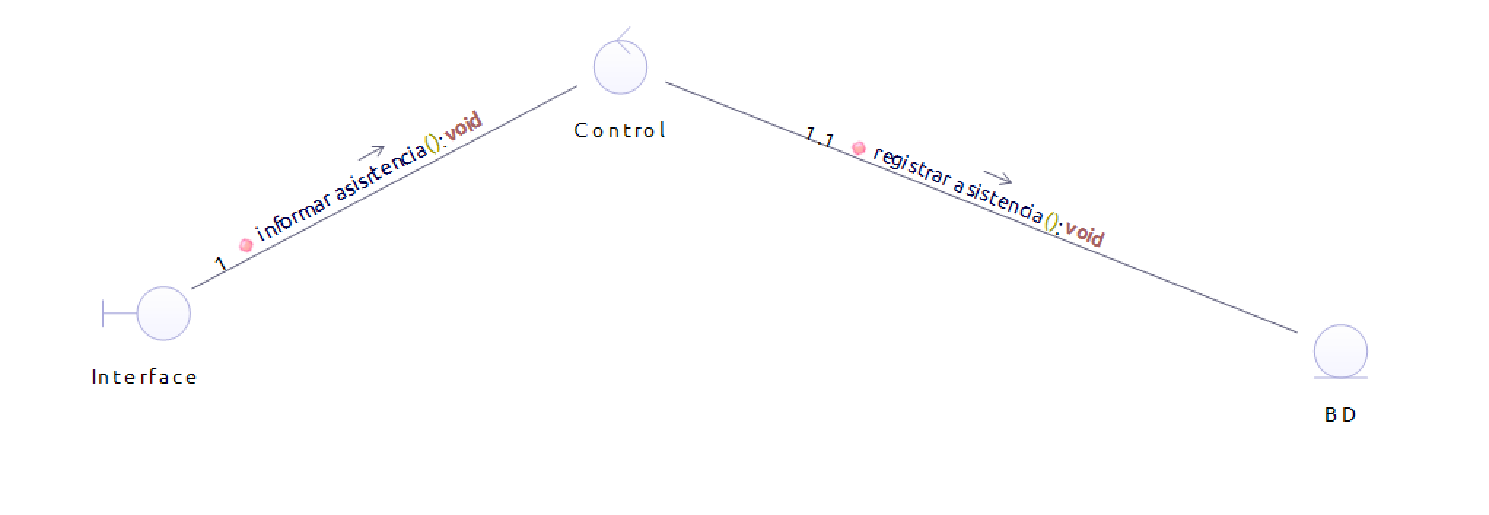
\includegraphics[width=1\linewidth]{parte2/imgs/DiagramaComunicacion/ComAsist}
	\caption[Diagrama de Comunicacion Control de asistencia]{Diagrama de Comunicación del control de asistencia}
	\label{fig:diagramaDeComunicacion}
\end{figure}

En la figura 4.6 la interfaz envia el mensaje "informar asistencia()" al objeto control que a su vez envia un mensaje "regisrarasistencia()" a la base de datos.


\newpage
%newpage para machetear y que no se vea tan paila

\paragraph{Diagrama del registro de usuarios}
\begin{figure}[H]
	\centering
	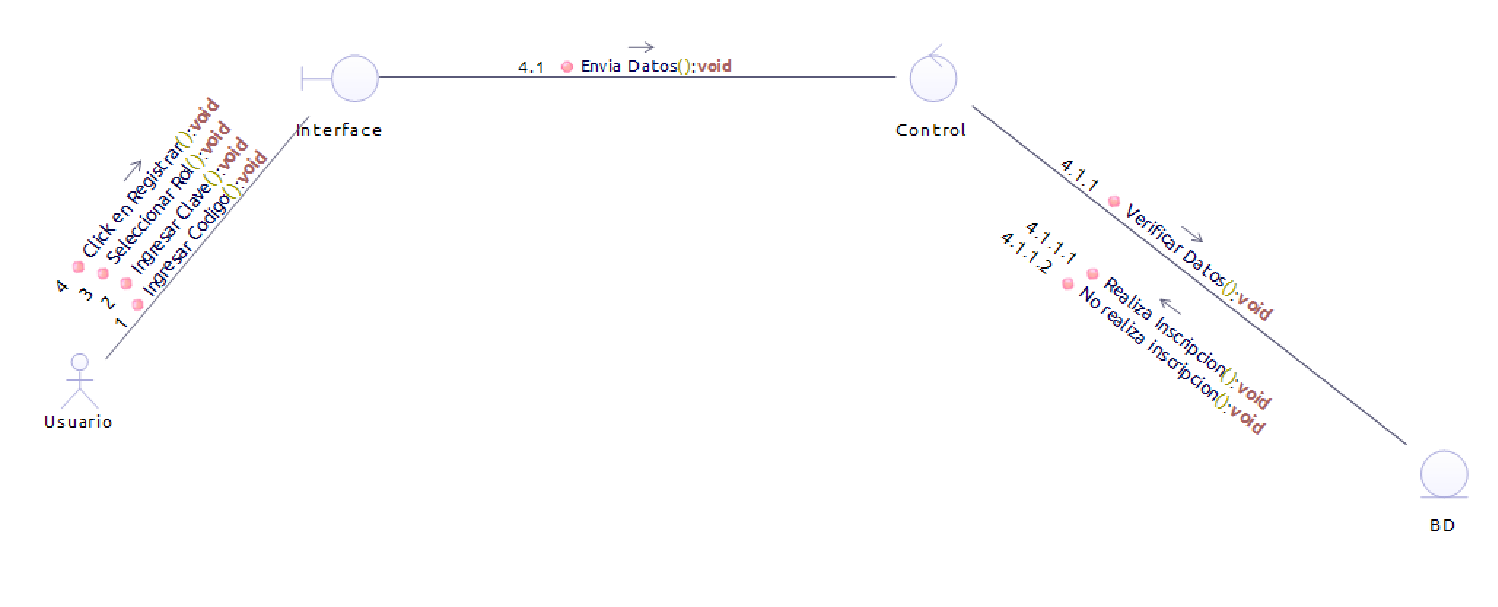
\includegraphics[width=1\linewidth]{parte2/imgs/DiagramaComunicacion/ComReguU}
	\caption[Diagrama de Comunicacion del registro de usuarios]{Diagrama de Comunicación del registro de usuarios}
	\label{fig:diagramaDeComunicacion3}
\end{figure}

En la figura 4.7 el usuario envia los mensajes "IngresarClave()", "IngrearCodigo()" a la interface,la interface envia el siguiente mensaje "EnviarDatos()"  al control 

\paragraph{Diagrama de la creacion de una convocatoria}
\begin{figure}[H]
	\centering
	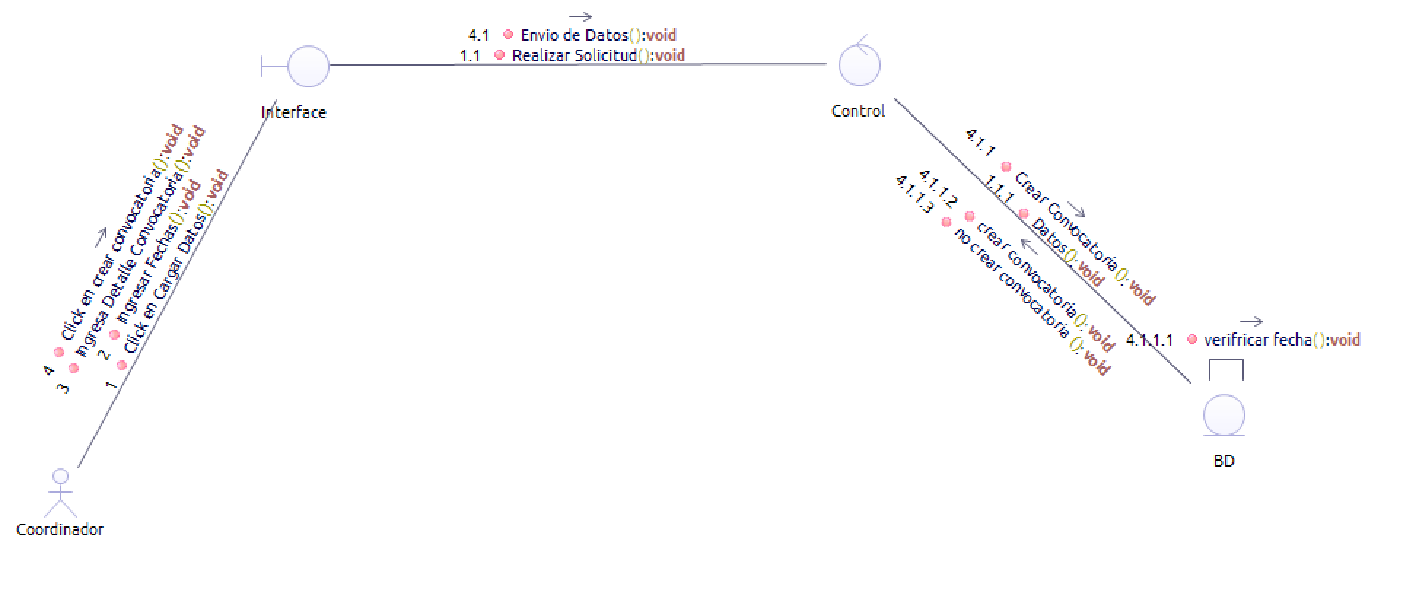
\includegraphics[width=1\linewidth]{parte2/imgs/DiagramaComunicacion/ComCreConv}
	\caption[Diagrama de Comunicacion cfracion Covoactoria]{Diagrama de Comunicación de la creacion de una convocatoria}
	\label{fig:diagramaDeComunicacion5}
\end{figure}

En la figura 4.8 el coordinador  envia los datos a la interfaz mediante el mensaje "cargarDatos()" y la interface mediante "EnvioDatos()" envia los datos a la base de datos y mediante "RealizarSolicitud()" envia datos de la solicitud a la base de datos, la base de datos recive "datos()" y se envia un mensaje de verificacion de datos "verificarfecha()".

\paragraph{Diagrama para la solicitud a una convocatoria}
\begin{figure}[H]
	\centering
	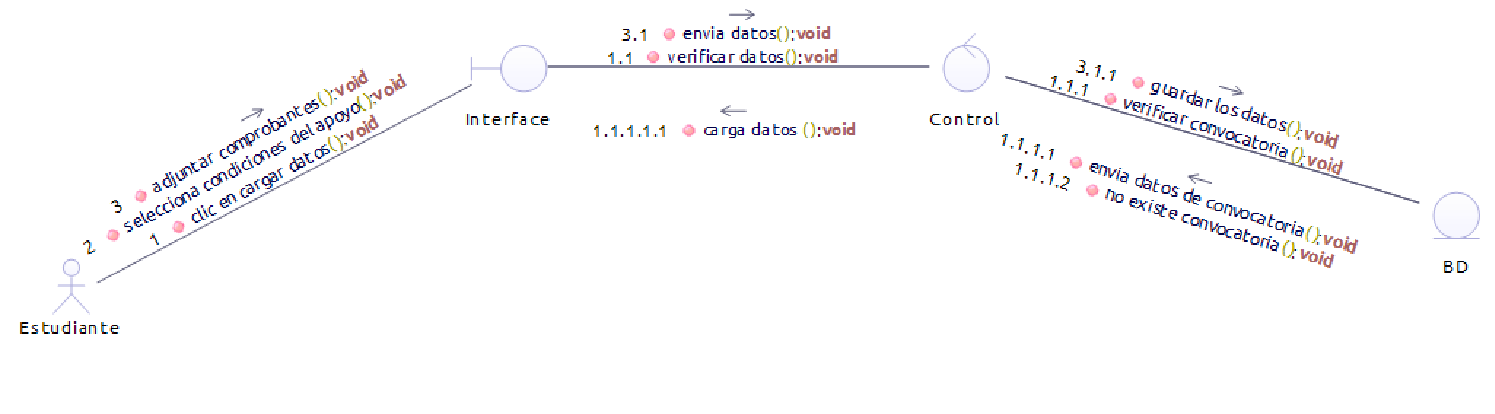
\includegraphics[width=1\linewidth]{parte2/imgs/DiagramaComunicacion/ComSoliConv}
	\caption[Diagrama de Comunicacion Solicitud a Convocatoria]{Diagrama de Comunicación para la solicitud a una convocatoria}
	\label{fig:diagramaDeComunicacion2}
\end{figure}

Para la figura 4.9  el estudiante envia los datos para la solicitud de la convocatoria a la interfaz y la interfaz envia y recive mensaje a la base de datos

\paragraph{Diagrama de la verificacion de una solicitud}
\begin{figure}[H]
	\centering
	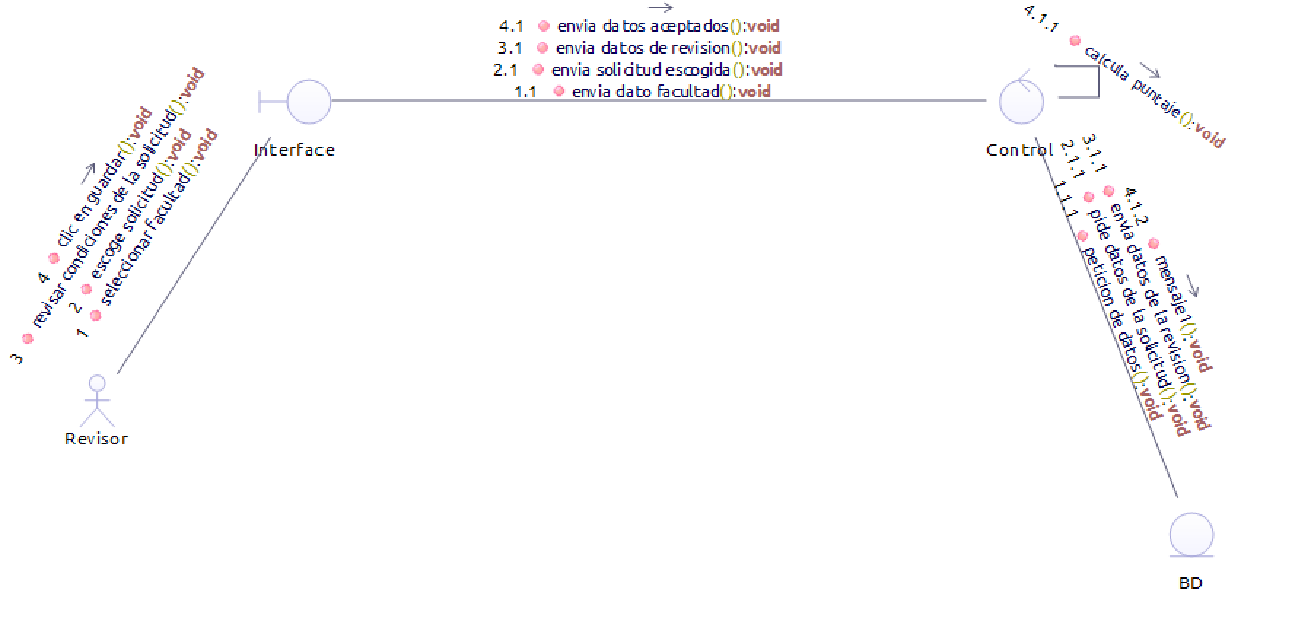
\includegraphics[width=1\linewidth]{parte2/imgs/DiagramaComunicacion/ComVer}
	\caption[Diagrama de Comunicacion verificacion solicitud]{Diagrama de Comunicación de la  verificacion de una solicitud}
	\label{fig:diagramaDeComunicacion4}
\end{figure}

Para figura 4.10 el revisor realiza las peticiones de las solicitudes mediante la interfaz a la base de datos y revisa los datos de los solicitantes para que despues se calcule el puntaje 

\newpage

%%%%%%%%%%%%%%%%%%%%%% Sección 4.3 %%%%%%%%%%%%%%%%%%%%%%%%%%%
\section{Diagramas de clases}

Para una análisis orientado al desarrollo del aplicativo se plantean los diagramas de clases, que básicamente representa la interacción entre distintas entidades que en conjunto logran cumplir con la funcionalidad del programa. Los diagramas de clases se componen principalmente de:

\begin{itemize}
	\item  \textbf{Clase}: Esta es la entidad que representara un objeto que interviene en la solución del problema. Su ilustración es un rectángulo dividido en 3 niveles: En el primero esta el nombre, el segundo es para los atributos y el ultimo es para las operaciones de dicho objeto
	\item \textbf{Relación}: Las relaciones se encargan de mostrar como es la interacción entre las clases de un diagrama, permite la comunicación entre las mismas y se dividen en 4 fundamentalmente
	
	
	\begin{itemize}
		\item \textit{\textbf{Herencia}}: Se encuentra en las clases cuando una clase "es una" clase aparte ya definida, en donde la herencia permite realizar una especialización, o en sentido inverso, hacer una generalización de unas características o comportamientos.
		\item \textit{\textbf{Dependencia}}: Se da cuando una clase depende de otra para su existencia o uso, pero la existencia de la primera no interfiere en la existencia de la segunda.
		\item \textit{\textbf{Asociación}}: Ocurre cuando una clase puede usar otra sin que sea obligatorio inicializarla al iniciar la clase principal
		\item \textit{\textbf{Composición}}: Es parecida a la asociación, sin embargo, esta relación hace obligatoria la inicialización de la clase agregada al momento de usar la clase principal.
	\end{itemize}
\end{itemize}

Haciendo uso de las clases y relaciones en un diagrama se puede llegar a una solución para el problema en un momento especifico en el tiempo, pero hay que tener en cuenta que el software debe poder perdurar en el tiempo de forma limpia, sin necesidad de hacer cambios como tal en el código existente sino solo permitir la adición de componentes o clases, para ello se usan los patrones de diseño que no son mas sino estructuras de clases y relaciones enfocadas solucionar los problemas del mantenimiento del software, mejorando así el ciclo de vida de la aplicación.

En los siguientes diagramas se mostraran algunos patrones de diseño en nuestra aplicación enfocados a distintos problemas al momento de plasmar la aplicación en un diagrama de clases.

\subsection{Creacionales}

\paragraph{Builder}
\begin{figure}[H]
	\centering
	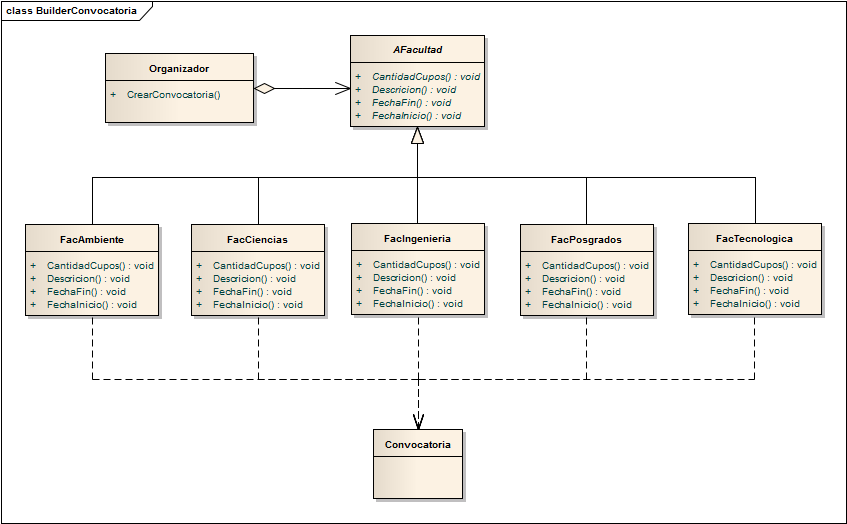
\includegraphics[width=1\linewidth]{parte2/imgs/Patrones/BuilderConvocatoria}
	\caption[Diagrama de clases del patrón Builder]{Diagrama de Clase para creación de de convocatorias por facultad}
	\label{fig:fabricaAbstracta}
\end{figure}

Como Patrón de diseño, el patrón builder (Constructor) es usado para permitir la creación de una variedad de objetos complejos desde un objeto fuente (Producto), el objeto fuente se compone de una variedad de partes que contribuyen individualmente a la creación de cada objeto complejo a través de un conjunto de llamadas a interfaces comunes de la clase Abstract Builder. En este caso la construccion se hace a travez de la creacion de convocatorias de cada facultad.


\paragraph{Factory}
\begin{figure}[H]
	\centering
	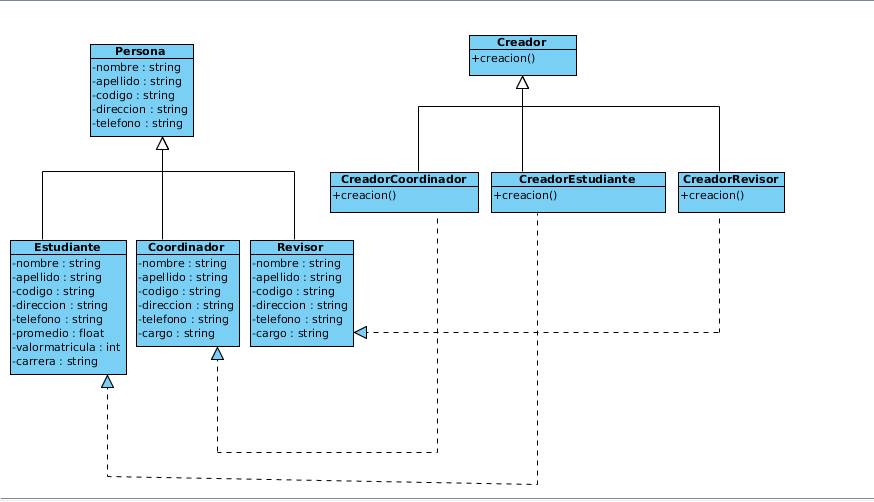
\includegraphics[width=1\linewidth]{parte2/imgs/Patrones/FactoryMethod}
	\caption[Diagrama de clases del patrón Facade]{Diagrama de Clase para el manejo de la conexión a distintas bases de datos a través del patrón de diseño Facade}
	\label{fig:facade}
\end{figure}

En diseño de software, el patrón de diseño Factory Method consiste en utilizar una clase constructora (al estilo del Abstract Factory) abstracta con unos cuantos métodos definidos y otro(s) abstracto(s): el dedicado a la construcción de objetos de un subtipo de un tipo determinado. Es una simplificación del Abstract Factory, en la que la clase abstracta tiene métodos concretos que usan algunos de los abstractos; según usemos una u otra hija de esta clase abstracta, tendremos uno u otro comportamiento. En esta caso implementamos el patron Factory Method para la creacion de diferentes personas que pueden ser estudiantes,coordinador y revisor ya que a pesar de ser hijos del mismo tipo las clases realizan distintas funciones en el software. 

\paragraph{Singleton}
\begin{figure}[H]
	\centering
	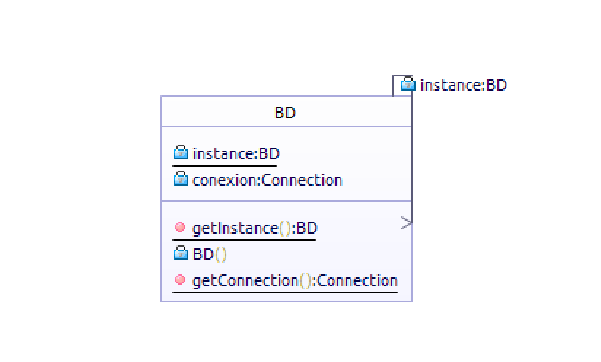
\includegraphics[width=1\linewidth]{parte2/imgs/Patrones/Singleton}
	\caption[Diagrama de clases del patrón Singleton]{Diagrama de Clase para el manejo de las operaciones de escritura/lectura sobre base de datos a través del patrón de diseño Bridge}
	\label{fig:puente}
\end{figure}

En ingeniería de software, singleton o instancia única es un patrón de diseño que permite restringir la creación de objetos pertenecientes a una clase o el valor de un tipo a un único objeto. Su intención consiste en garantizar que una clase sólo tenga una instancia y proporcionar un punto de acceso global a ella.El patrón singleton se implementa creando en nuestra clase un método que crea una instancia del objeto sólo si todavía no existe alguna. Para asegurar que la clase no puede ser instanciada nuevamente se regula el alcance del constructor (con modificadores de acceso como protegido o privado). En este caso aplicamos este patron para controlar el acceso a la base de datos.

\subsection{Comportamiento}

\paragraph{Iterador}
\begin{figure}[H]
	\centering
	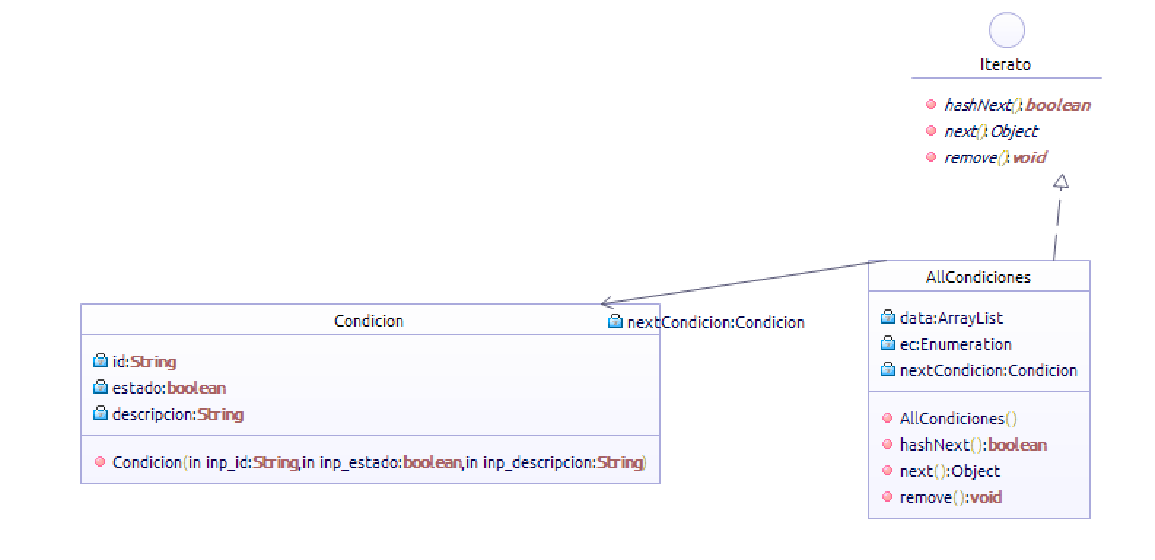
\includegraphics[width=1\linewidth]{parte2/imgs/Patrones/Iterador}
	\caption[Diagrama de clases del patrón Iterador]{Diagrama de Clase para la ejecucion de acciones de CRUD mediante el patron de diseño Comando}
	\label{fig:command}
\end{figure}

Proporcionar una forma de acceder a los elementos de un objeto agregado de forma secuencial sin exponer sus detalles. En este caso me permite analizar todas las condiciones que hay para evaluar el puntaje de la solicitud al apoyo alimentario.



\paragraph{State}
\begin{figure}[H]
	\centering
	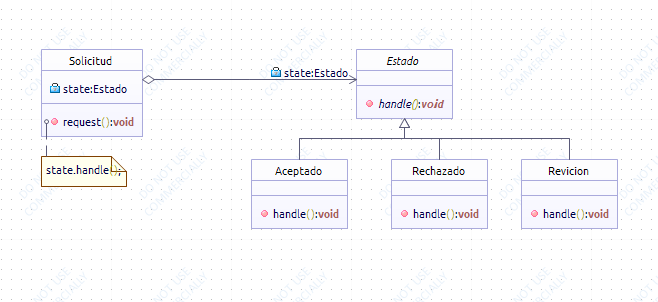
\includegraphics[width=1\linewidth]{parte2/imgs/Patrones/Estado}
	\caption[Diagrama de clases del patrón State]{Diagrama de Clase para la relacion entre flujos financieros y sugerencias mediante el patron de diseño Mediator}
	\label{fig:mediador}
\end{figure}
El patrón de diseño State se utiliza cuando el comportamiento de un objeto cambia dependiendo del estado del mismo. Por ejemplo: una alarma puede tener diferentes estados, como desactivada, activada, en configuración. En este caso permite manejar el estado el cambio de una solicitud de aceptado, rechazado y revicion.

